\documentclass[a4paper,12pt]{article}
\usepackage{graphicx}
\usepackage[T
1]{fontenc}
\usepackage{parskip}
\usepackage{latexsym,amsmath,amssymb}
\usepackage{natbib}
\usepackage{times}
\usepackage{zi4}
\usepackage[a4paper,left=3cm,right=3cm,top=3cm,bottom=3cm]{geometry}
%\usepackage{foundrysterlingbookosf}
\usepackage{setspace}

% Turn off page numbering until first section.
\usepackage[utf8]{inputenc}
\usepackage{tikz-cd}
\usepackage{biblatex}
\usepackage{amsmath}
\addbibresource{refs.bib}
\usepackage{multirow}
\usepackage{subcaption}
\usepackage{mwe}
\usepackage{caption}
\usepackage{multirow}
\usepackage{booktabs}
\usepackage[normalem]{ulem}
\DeclareMathOperator*{\argmax}{arg\,max}
\DeclareMathOperator*{\argmin}{arg\,min}
\usepackage{xcolor}
\usepackage{wrapfig}
\usepackage{hyperref}
\usepackage{threeparttable}
\usetikzlibrary{decorations.pathreplacing}
\usetikzlibrary{positioning}
\captionsetup[table]{labelfont=bf}
\captionsetup[figure]{labelfont=bf}
\usepackage{longtable}
\usetikzlibrary{shapes,decorations,arrows,calc,arrows.meta,fit,positioning}
\tikzset{
    -Latex,auto,node distance =1 cm and 1 cm,semithick,
    state/.style ={ellipse, draw, minimum width = 0.7 cm},
    point/.style = {circle, draw, inner sep=0.04cm,fill,node contents={}},
    bidirected/.style={Latex-Latex,dashed},
    el/.style = {inner sep=2pt, align=left, sloped}
}
% credit: https://dkumor.com/posts/technical/2018/08/15/causal-tikz/
\usetikzlibrary{shapes.geometric, arrows.meta, positioning, decorations.pathreplacing}
\author{Salim Damerdji}
\date{August 2023}

\usepackage{graphicx} % Required for inserting images

\title{Estimating the Effect of San Francisco's Impact Fees on Housing Production \thanks{My deepest thanks to Professor Frank Windmeijer for his thoughtful guidance and invaluable feedback. And a warm thank you to Reza Amindarbari of San Francisco Planning for his generous help in explaining and providing data from the City. Many thanks to Professor Chris Elmendorf and Dr. Issi Romem for their kind verbal feedback and wise advice when I first set out to pursue this paper.}}
\author{Salim Damerdji}
\date{September 2023}
\begin{document}
\onehalfspacing
\maketitle
\begin{abstract}
Housing shortages across the country have raised rents and displaced tenants, putting housing policy on the agenda at the state and local level. Yet, policymakers lack visibility into how much housing would get built under alternative proposed reforms. This paper analyzes the causal effect of reducing impact fees on housing production and finds that even a 50\% reduction in impact fees may fail to push the needle on housing production. Using San Francisco as a case study, I analyze adjacent parcels where one parcel is subject to a 50\% higher impact fee than its neighboring parcel. Over a 2014-2023 timeframe, I find no difference in the probability of development of adjacent lots, no difference in the expected unit count conditioned on development occurring, and, by consequence, no difference in housing production. This result is corroborated by a Double/Debiased Machine Learning algorithm that uses machine learning to control for nearly one hundred parcel-specific factors and their non-linear interactions. Policy-makers motivated to promote housing production should identify policy solutions that do more than reduce impact fees - like those under study - by 50\%.
\end{abstract}
\renewcommand{\arraystretch}{1.5}
\vspace{5}
\textbf{Keywords:} Housing Supply, Spatial Econometrics, RDD, Double/Debiased ML
\clearpage
\section{Introduction}

In high-demand cities, new housing construction reduces rents.\cite{pennington2021does}\cite{mense2020impact}\cite{li2022new}\cite{asquith2019supply}\cite{mast2019effect}\cite{glaeser2018economic} To redress regional housing shortages,\cite{herkenhoff2018tarnishing} policymakers nationwide are contemplating proposals to increase housing production.\cite{wegmann2020death} Yet, there are as many policy levers to produce more housing as there are regulations that currently constrain housing production, of which there are many.\cite{bronin2023zoning}\cite{herkenhoff2018tarnishing} Policymakers motivated to tackle housing shortages, thus, face a prioritization question: given a slew of possible reforms, which reforms should be prioritized? A twin question is: which reforms match the scale of the housing crisis? 

One policy option is to reduce impact fees. An impact fee is a financial exaction that local jurisdictions levy on new development to pay for the costs of public services associated with new development.\cite{been2005impact} Though property taxes and other local taxes historically paid for infrastructure, cities starting in the 1920s gravitated towards using impact fees to pay for a wider and wider scope of infrastructure.\cite{been2005impact} In California, impact fees now can add tens of thousands of dollars to the cost of development for each unit of an apartment, though the figure ranges widely from city to city.\cite{mawhorter2018all} Typically, cities require impact fees to be paid before the apartment is built, which means that high-interest loans compound the costs of these fees.\cite{raetz2019residential}\cite{phillips2021reducing}

Reducing impact fees lowers the cost of development and should, in theory, spur housing production. The strength of this relationship, however, remains an open question. The existing literature primarily focuses on the relationship between impact fees and the affordability of housing, and most studies find that impact fees raise housing prices.\cite{evans2003effects} But the focus on home prices side-steps an essential question: do prices rise because of decreased supply or increased demand?\cite{mayer2000land} The latter possibility is raised by authors who hypothesize that impact fees increase demand for neighborhoods by paying for amenities that otherwise would not exist - or would only otherwise exist with increased property taxes.\cite{been2005impact} 

Existing research on the causal effect of impact fees on housing supply is sparse and mixed. Skidmore and Peddle studied a panel dataset from 1977 to 1992 in DuPage County, Illinois, and the authors found a 25\% reduction in the rate of housing development for cities that had an impact fee.\cite{skidmore1998development} Using a richer, nationwide dataset, Mayer and Somerville find no statistically significant relationship between impact fees and housing production.\cite{mayer2000land}

This paper contributes to this literature by proposing a novel identification strategy. Using San Francisco as a case study, I compare neighboring parcels of land where one parcel is subjected to a 50\% higher impact fee than its neighboring parcel. I control for selection bias by using a rich parcel-level dataset that describes how these parcels are zoned, what's built on each parcel, whether the landowner has recently made improvements, and so on. (See \textbf{Table \ref{tab:data.sources}} in the Appendix for the extended list.) If controlling for this large set of variables is insufficient to control for selection bias, I argue that any unobserved sources of selection bias vary continuously along the border between two neighboring parcels subject to different fees. To make this concrete, \textbf{Figure \ref{fig:eg_boundary}} provides a street view of this boundary; my assumption is that, if there are unobserved confounders, that their effect on housing production varies smoothly across the boundary. For example, if local opposition to housing both causes higher impact fees and reduces housing production, then my assumption is that a local community group would be similarly opposed to housing developments on neighboring parcels separated by the fee boundary.\footnote{To be precise, the success of the identification strategy does not hang on whether the local opposition is equivalent on either side of the boundary: I merely need that the degree of opposition does not drop off suddenly at the boundary. With other words, identification requires that unobserved confounders vary continuously at the boundary.} If this assumption holds, then by framing the boundary between these parcels as a sharp, geospatial regression discontinuity, I can show that, after controlling for observed variables, any discontinuity in housing production is caused by the impact fees.

\begin{figure}[hpbt]
\centering
    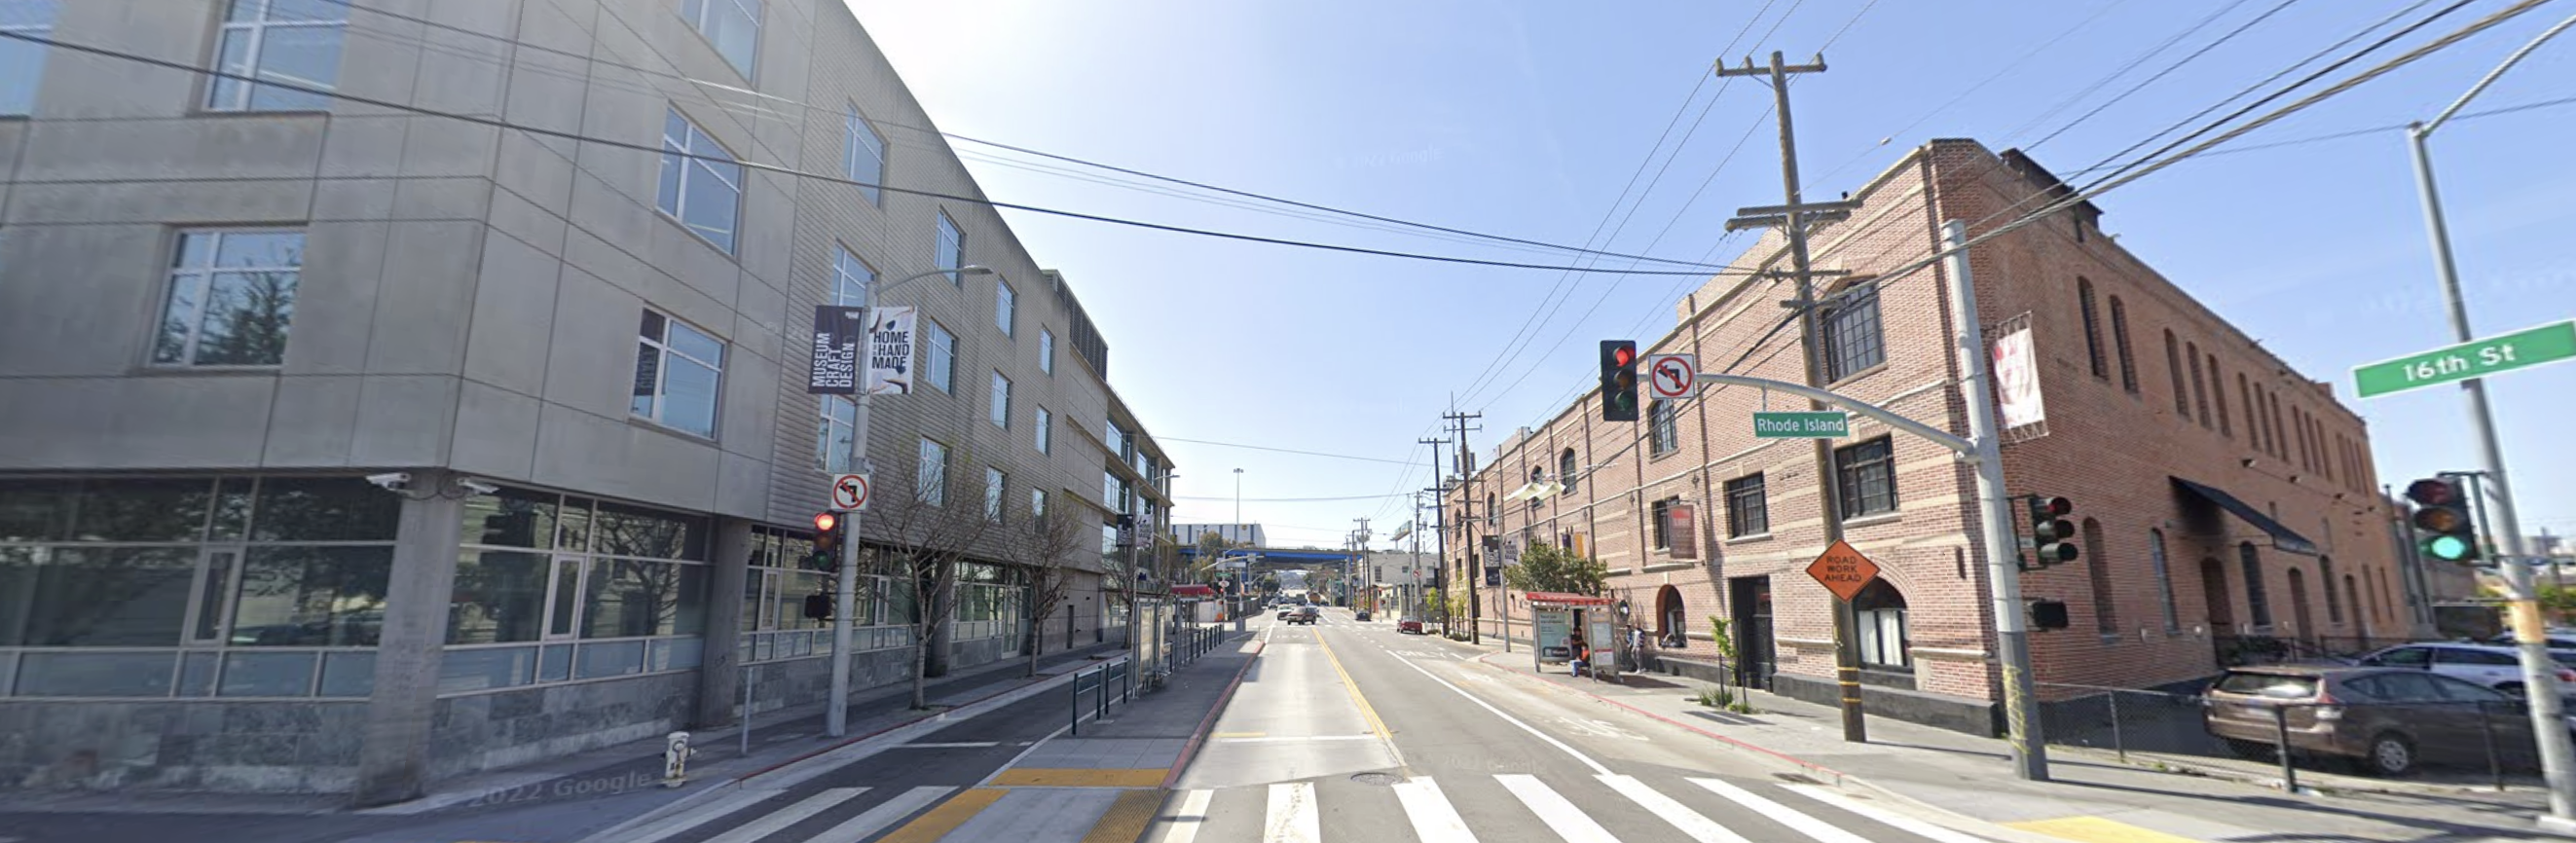
\includegraphics[scale=.3]{figures/boundary_eg.png}
    \caption{Example of two neighboring parcels on the boundary.}
    \label{fig:eg_boundary}
\end{figure}

The impact fees in question regulate development in four neighborhoods in San Francisco: South of Market (SoMa), the Mission, the Showplace Square/Potrero Hill neighborhood, and the Central Waterfront. The City and County of San Francisco refers to these four neighborhoods as the Eastern Neighborhoods for shorthand. Starting in 2011, the City implemented policies to encourage housing construction in these neighborhoods. In the last decade, 32\% of all units built in San Francisco have been built in these four neighborhoods. 

Pursuant to the Mitigation Fee Act of 1987, San Francisco conducted a Nexus Study in 2008, which found that new development would require additional expenditures to pay for library expansions, childcare facilities, transit infrastructure, and parks.\cite{SFPlanning2008} Rather than charge all development at the highest amount legally allowed by the Nexus Study, the City opted to charge higher impact fees - which the City refers to as Tier 2 fees - to parcels that were upzoned more as part of the area plan updates. Most parcels in these neighborhoods, however, are subjected to a lower impact fee, which the City refers to as the Tier 1 fee. Both fees are charged on net new square footage built for residential use. Annual fees increases are indexed to the Annual Infrastructure Construction Cost Inflation Estimate. As of 2023, the lower impact fee costs \$14.72 per square foot, and the higher impact fee, which is indexed to cost 50\% more, is \$22.08 per square foot.\cite{SF_ImpactFeeRegister_2022} For a prototypical 100-unit apartment building, this raises the per-unit development cost by \$7,500.\footnote{These calculations are derived from a 2022 pro-forma kindly provided by a developer in SF.} That's about 0.8\% of the total development costs and, after accounting for high interest loans used to pay the fee, the fee and the additional interest incurred may account for 1.2\% of total development costs for a prototypical project.\cite{phillips2021reducing}



\begin{figure}[hbt]
    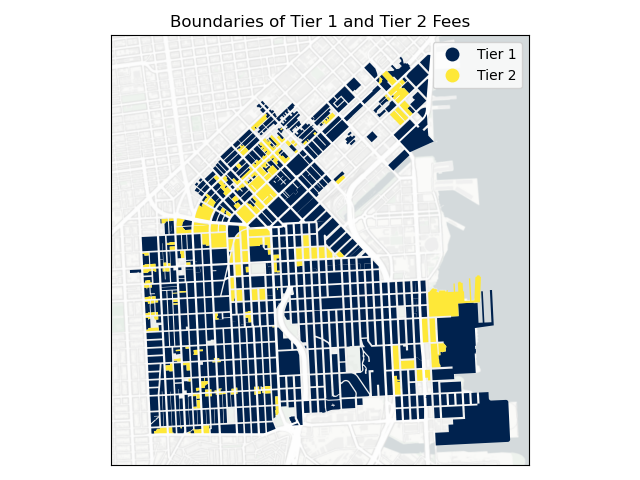
\includegraphics[scale=.8]{rdd/tier1_tier2_boundaries.png}
    \caption{Parcels in yellow are subject to a 50\% higher impact fee than parcels in dark blue.}
    \label{fig:tier1_tier2_boundaries}
\end{figure}


This paper addresses two difficulties in studying parcel-level housing production in this case study. First, geospatial regression discontinuity designs (RDD) frequently involved compounding treatments at the border,\cite{keele2015geographic} and that is the case with these impact fees under study. As explained earlier, San Francisco imposes higher fees on parcels that benefitted more from upzoning during the 2011-2014 time period. As a result, estimates of the effect of the impact fee will be biased unless one controls for the effect of zoning on the parcel. Yet, if one only models the effect of zoning based on parcels near the fee boundary under study, the zoning and fee variables will, of course, be highly collinear, and so the fitted coefficients will be unstable, with large standard errors. I solve this challenge by relying on a unique source of data that provides helpful simplifications of San Francisco's zoning codes for 153,010 parcels citywide. By using parcels from across the city to estimate the contribution of zoning to housing production, I am able to decrease the variance of my estimates and, by consequence, adequately control for this compounding treatment.


The second challenge I face is in modelling housing production.  Typical count data models like Poisson regression will not suffice for modelling housing development for two reasons: first, the factors that determine \textit{whether} housing is built overlap with, but are not identical to the factors that determine \textit{how much} housing will get built if anything is. For example, if a parcel has a dilapidated building on it, that increases the probability of development occurring, but there's no obvious reason as to why the existing use would affect how much housing is built, if any. For standard count data models, there is no separate way to model zeroes from positive counts, but modelling these two phenomena separately would likely improve one's ability to model housing production. The second limitation of conventional count data models is that there's overdispersion in the data: on most parcels, nothing is built; on a tiny fraction of parcels, most of the City's new housing is built. As a result, there are more undeveloped parcels and also more intensively-redeveloped parcels in the data than a Poisson or negative binomial distribution would predict. Both of these shortcomings are addressed by using a hurdle model that, firstly, uses logistic regression to model the probability of development occurring and, secondly, uses Poisson regression to model how many homes would be built on a parcel, if it's developed. 

Using a hurdle model also provides an additional interpretive benefit in that it disaggregates overall housing production into its two component factors: a parcel's probability of development $\mathbb{P}[D]$, and a parcel's expected unit count if developed, $\mathbb{E}[U|D]$. This disaggregation is useful for policymakers because, while pro-supply policymakers may be agnostic as to which lever to pull, some policymakers prefer to increase $\mathbb{E}[U|D]$, but not $\mathbb{P}[D]$, for concern of development displacing tenants, while other policymakers may prefer to increase $\mathbb{P}[D]$, not $\mathbb{E}[U|D]$, by way of an aesthetic preference for views where no one building sticks out. 

Contrary to Skidmore and Peddle, my findings ultimately agree with the null findings from Mayer and Somerville. Using a geospatial RDD with a hurdle model, I find no difference in the probability of development of neighboring lots subjected to different fees, no difference in the expected unit count conditioned on development occurring, and, taking these results together, no difference in overall housing production. My findings represent a conservative estimate of the causal effect of the impact fees because, by construction, I do not allow for the possibility that the impact fees were necessary to make the upzonings on the eastern side of the city politically feasible.


To confirm that this result does not stem from parametric modelling assumptions, I perform a robustness check with Double/Debiased Machine Learning, which uses machine learning to control for nearly one hundred parcel-specific factors and their potentially complex non-linear interactions. This robustness check corroborates the same basic story that a 50\% reduction in fees does not register as a statistically significant constraint removal.

My findings indicate that policymakers motivated to increase housing supply should prioritize other housing reforms over impact fee reform. While there is much variation in impact fees from city to city, and there are surely some cities successfully leveraging impact fees in an exclusionary way, impact fee reforms are unlikely to prompt much, if any, housing production in a city like San Francisco.

\section{Data}
\subsection{Sources}
\label{data.sources} 


This project merges six data sources provided by the City and County of San Francisco with neighborhood-level home price data.

The treatment variable of interest comes from San Francisco's Neighborhood-Specific Impact Fee Areas dataset, a geospatial dataset of fees charged for residential development in some parts of the city but not others.

The outcome of interest - how much housing was built on a parcel - came from San Francisco's Department of Building Inspection's (SF DBI) dataset of permits, which indicates the date a permit was created, how many homes were built, and where they were built. Specifically, I filtered for relevant SF DBI permits based on the latest available list of completed housing developments from San Francisco's Planning Department.\footnote{This data was generously provided by SF Planning Department's Reza Amindarbari, a manager in the Data \& Analytics Group, via private correspondence in July 2023.}

I joined this dataset with San Francisco's BlueSky dataset, which tracks roughly 150,000 San Francisco parcels from 2001 to 2016 and includes information on each parcel's historical status, residential status, the existing building envelope, and the potential buildable envelope given the parcel's zoning designation.\cite{SFHousingElement2022AppendixB} When the City prepared the BlueSky dataset, they removed duplicative parcel identifiers, including condos, and they removed parcels with no potential for residential capacity (such as parks). This dataset provides several variables that a priori are predictive of where housing will get built: parcels listed as a historical resource are harder to redevelop into housing due to California's Environmental Quality Act; parcels that have existing homes with tenants are harder to redevelop due to San Francisco's tenant protections that make demolitions costly; and the parcel's zoning determines how much revenue can be gained by redeveloping the parcel, as more square footage can be built with looser zoning. As a result, controlling for these variables improves the precision of my estimate.

This dataset is joined with data from the county tax assessor, which includes information on the age of the property, the construction type, the property's square footage, the basement area, lot area, lot shape, the ownership status, the prior sale date of the land, the assessed improvement value, the assessed land value, the number of bedrooms, baths, stories, and units, and more.  

Because steep lots pose unique construction costs, I join this dataset with a topological map of San Francisco. Created in 2019, this dataset is post-treatment but causally unaffected by the treatment, while strongly predicting development. Thus, its inclusion increases the precision of my estimate.

Finally, I incorporate lag indicators for whether the landowner applied for a permit for each parcel to build, tear down, improve, or alter something on the parcel by joining the panel dataset with SF DBI's dataset of permits. A priori, one would think that permits to improve a parcel are negative indicators that the owner is interested in tearing down the property to rebuild. Conversely, it is reasonable that demolition permits are lead indicators for future development on the parcel.

The economic feasibility of building homes depends strongly on neighborhood rents, and so I join my dataset with Zillow's Home Value Index for All Homes (both single family and condos) for annual rent per neighborhood in San Francisco.\footnote{This is the only neighborhood-level data provided by Zillow.}

In all, there are nearly a hundred covariates in addition to the treatment and outcome.  Key explanatory variables are presented in \textbf{Table \ref{tab:data.sources}} in the Appendix.

\subsection{Cleaning}

All but two of the aforementioned datasets are geospatial. That is, for most of my sourced datasets, each observation is accompanied by a set of coordinates that indicates the observation’s shape and location on a map, as well as a Coordinate Reference System (CRS) for identifying which map. For consistency and accuracy, I translate all geospatial datasets to the California Albers transformation of North American Datum of 1983, a coordinate reference system which minimizes errors in estimating the distance of points in California.

To dovetail the datasets together, I primarily relied on geospatial joins through the Python package geopandas. Two joins had to be handled differently because two sourced datasets lacked geospatial information: San Francisco’s BlueSky dataset and the Zillow dataset on neighborhood-level home prices. For SF’s BlueSky dataset, I joined this dataset using the block lot parcel identifier with San Francisco’s geospatial dataset of all active and retired parcels, thus yielding a geospatial version of the BlueSky dataset. For Zillow’s neighborhood-level home price dataset, performing a join was non-trivial since there was no equivalent geospatial dataset containing all and only the neighborhood names in Zillow’s historical home price dataset. Instead, the best I could find was a 2011 Zillow geospatial dataset of neighborhoods via the WayBack Machine, which did not match up exactly with the neighborhoods now used by Zillow’s neighborhood-level home price dataset in 2023. To reduce the number of parcels with missing values for local home values, I first performed the join based on how the tax assessor lists the neighborhood, a join which succeeds for most parcels in my panel dataset, and then used the geospatial information for a join where missing values remained.

\section{Exploratory Data Analysis}

Homebuilding is relatively rare. In the decade under study, there are 1,970 parcels where housing is built in a dataset of 153,010 parcels. Because 98.7\% of all parcels see no development, the dataset contains an inflated number of zeros relative to a Poisson distribution. When housing is built, most housing projects add just one or two homes, but a few housing projects make up the bulk of what the city builds, as indicated by \textbf{Table \ref{tab:NetUnitsCompleted}}. The five largest projects alone account for more units built than the 1393 single-unit projects. To inform policy-makers about the supply effects of potential policies, it is plainly important, therefore, to not just model how policies affect the rate of development, but also the size of the projects that are built.


\begin{table}[hbt]
\centering
\caption{Number of Observations for Different Buckets of Residential Project Size}
\setlength{\tabcolsep}{10pt} 
\begin{tabular}{r|cccccccccccc}

\hline
\textbf{Units Built} & 1 & 2 & 3 & 4 & 5-10 & 11-199 & 200-399 & 400+ \\
\hline
\textbf{Count} & 1393 & 255 & 85 & 48 & 55 & 116 & 15 & 3 \\
\hline
\end{tabular}
\label{tab:NetUnitsCompleted}
\end{table}


Development trends vary dramatically across San Francisco. \textbf{Figure \ref{fig:eda_spatial_trend}} shows where housing gets built. Each purple circle reflects a housing development, with the size indicating how many units of housing were built as part of the development: large circles reflect large apartment (or condo) complexes. As can be seen, most of the total units built are built on the east side of the city. The west side of the city, in comparison, sees development, but of a very different type: namely, accessory dwelling units. Much of this variation is downstream of zoning, which underscores why it is important to control for zoning capacity in estimating the effect of impact fees, as argued in Section \ref{data.sources}.


\begin{figure}[hbt]
    \centering
    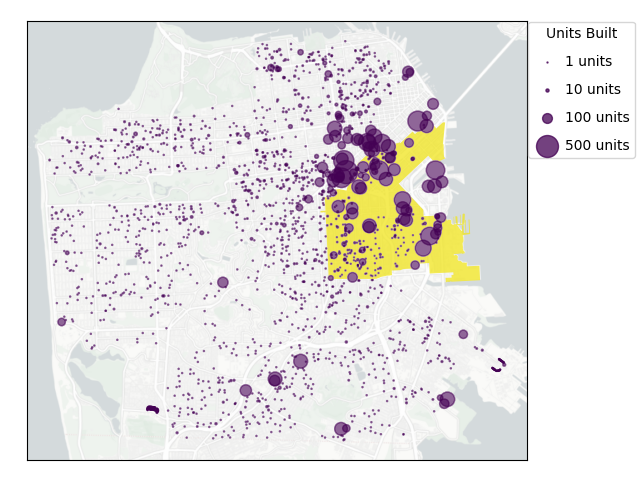
\includegraphics[scale=.75]{./rdd/figures/where_housing_gets_built2014.png}
    \caption{Spatial trends in homebuilding. The four neighborhoods - SoMa, Mission, Central Waterfront, and Protrero Hill - are shaded in yellow.}
    \label{fig:eda_spatial_trend}
\end{figure}

In \textbf{Figure \ref{fig:eda_barplots}}, there is evidence that properties with existing single family residences and government uses are less likely to be redeveloped into housing. Furthermore, it's striking that parcels with an existing use that's categorized as Miscellaneous/Mixed-Use are much more likely to be developed into housing, at roughly three times the rate of other parcels. 

\begin{figure}[hbtp]
    \centering
    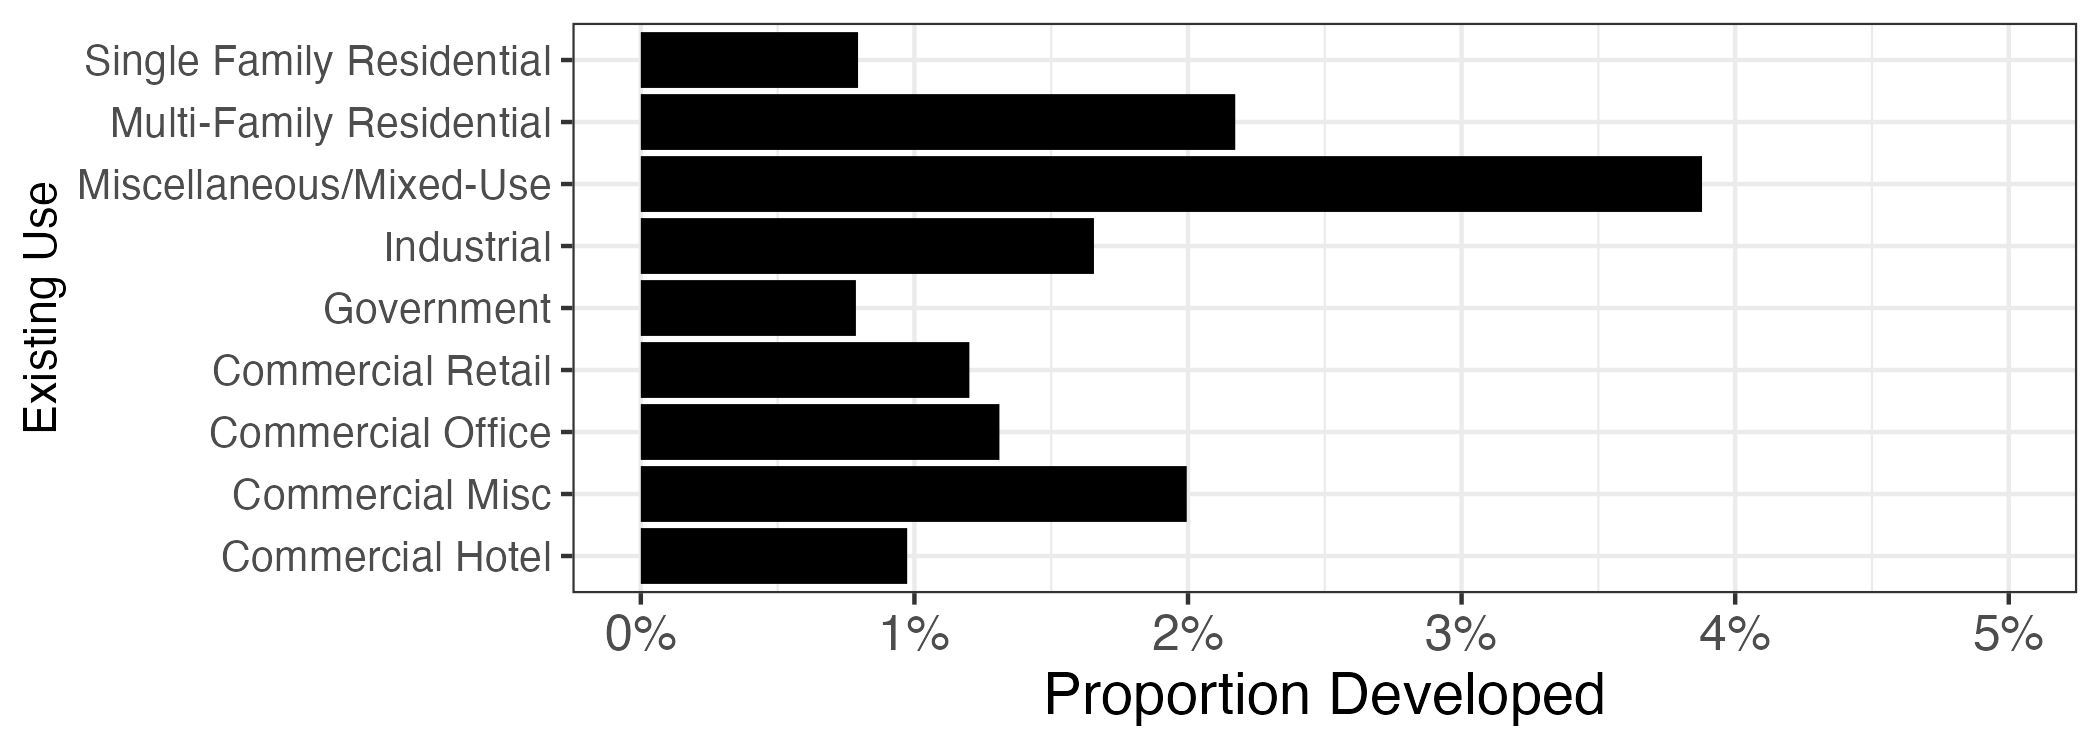
\includegraphics[scale=.85]{./figures/eda_barplots.png}
    \caption{Development rates of parcels based on the existing use.}
    \label{fig:eda_barplots}
\end{figure}


Per \textbf{Table \ref{tab:correlation_with_developed}}, most variables are weakly correlated with whether or not housing is built. The variables displayed are those whose pearson correlations have the largest absolute values, and so most variables have virtually no correlation at all with whether housing is developed. A priori, however, one should not expect strong linear, univariate relationships between these variables and development for the simple reason that development is mediated by financial metric analyses that involve the non-linear interaction of half a dozen variables, including rent, land values, zoning, and various neighborhood-level factors like impact fees.\cite{la}\cite{metcalf2021will}




\renewcommand{\arraystretch}{1}

\begin{table}[hbt]
\centering
\caption{Pearson Correlation Coefficients with Binary Indicator for Development}
\setlength{\tabcolsep}{10pt} 
\begin{tabular}{r l}
\hline
\textbf{Variable} & \textbf{Correlation with Development} \\
\hline
Year Property Built & -0.055 \\
4+ Unit Zoning & 0.045 \\
Homeowner Exemption Value & -0.044 \\
Form-Based Zoning & 0.035 \\
Upzone Ratio & 0.031 \\
\hline
\end{tabular}
\label{tab:correlation_with_developed}
\end{table}
\renewcommand{\arraystretch}{1.5}

Given that housing is built, a slightly different set of factors are relevant to how much housing is built, as outlined in \textbf{Table \ref{tab:correlation_with_count_homes}}. For example, the top two variables are both functions of the square footage that can built on a parcel: buildable envelope is the square footage permitted under the City's zoning; and revenue is the product of the buildable envelope and neighborhood rent per square foot. This is trivially what we would expect to see.

\renewcommand{\arraystretch}{1}
\begin{table}[hbt]
\centering
\setlength{\tabcolsep}{10pt} 
\caption{Pearson Correlation Coefficients with Count of Homes Built on Parcel, Conditioned on Development}
\begin{tabular}{r l}
\hline
\textbf{Variable} & \textbf{Correlation with \# of Homes Built} \\
\hline
Revenue & 0.612 \\
Buildable Envelope & 0.545 \\
Existing Residential Use & -0.455 \\
Office/Commercial Zoning & 0.438 \\
Lot Area & 0.425 \\
\hline
\end{tabular}
\label{tab:correlation_with_count_homes}
\end{table}
\renewcommand{\arraystretch}{1.5}


The disparity in which variables are correlated with development as opposed to units built, again, motivates the view that the decision to build housing is a separate decision from the choice of how much housing to build. For example, it's intuitive that the historical status of a building affects \textit{whether} a parcel is redeveloped, but less so how much housing is built, conditioned on there being development. A parcel's historical status adds expensive CEQA red tape to build anything, but that red tape does not scale linearly as the unit count increases.

Turning our attention to the four eastern neighborhoods under study, it's helpful to look at how certain key variables vary near the border between two fees. A histogram breaks down the distribution of parcels with Office/Commercial Zoning in \textbf{Figure \ref{fig:office_zoning_boundary}}. The histogram bars plotted to the left of zero are those where the lower fee is paid, and the bars to the right of zero reflect parcels where the higher fee is paid. Clearly, the two groups are very unalike as a whole: there's much more office zoning for the parcels subject to the higher fee (those to the left of 0) than for the parcels subject to the lower fee (those to the right of 0). However, along the border, parcels are zoned much more similarly. For this reason, I estimate the effect of the higher fee only by comparing those parcels just along the boundary.

\begin{figure}[hbtp]
    \centering
    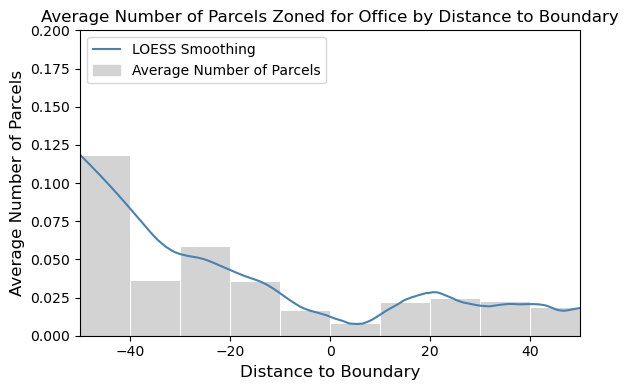
\includegraphics[scale=.8]{rdd/office_zoning_boundary.png}
    \caption{RDD Boundary versus Important Predictor, Office Zoning.}
    \label{fig:office_zoning_boundary}
\end{figure}

Using a 5 meter threshold for the distance between any two neighboring parcels, the parcels selected to estimate the local average treatment effect are shown in \textbf{Figure \ref{fig:subset}}. In all, 1,043 neighboring parcels are selected to estimate the effect of the fees on housing production. Of these parcels, 594 are subject to the lower fee, and 449 are subject to the higher fee.

\begin{figure}[hbtp]
    \centering
    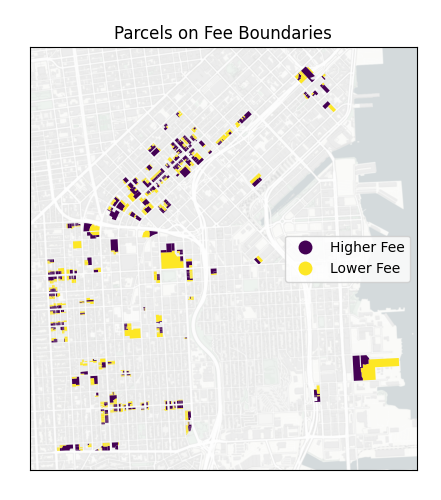
\includegraphics[scale=.8]{rdd/figures/eastern_fees.png}
    \caption{Parcels matched across the boundary.}
    \label{fig:subset}
\end{figure}

Even among this subset of parcels, however, there is known compounding treatment because these neighborhoods were selected to receive additional upzoning, which is why the parcels are subject to higher impact fees. Evidence of this compounding treatment is provided in \textbf{Figure \ref{fig:Envelope_boundary}}. Thus, not all covariates vary continuously along the fee boundary. To avoid obtaining biased estimates, an adequate model must, at minimum, control for variables that are a function of zoning.


\begin{figure}[hbt]
    \centering
    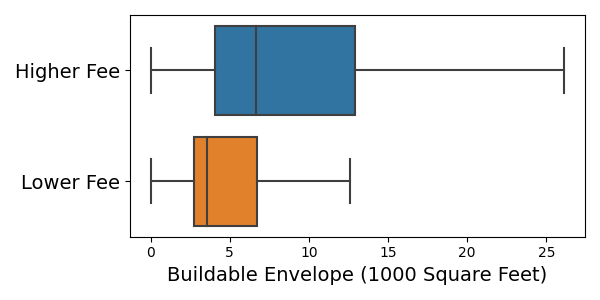
\includegraphics[scale=.7]{figures/Envelope_boundary.png}
    \caption{Comparing parcels within five meters of the fee boundary, parcels with a cheaper fee have stricter zoning than parcels with the more expensive fee.}
    \label{fig:Envelope_boundary}
\end{figure}


\section{Method}

I will refer to the higher fee - the second tier fee - as the treatment variable $F$. The average treatment effect is, then, the average difference in potential housing built if a parcel in the Eastern Neighborhoods is subjected to the higher fee instead of the lower fee.

The boundaries can be viewed as discontinuities in a sharp regression discontinuity design. I will estimate the local average treatment effect of the higher fee $F$ at a discontinuity. The treatment $F$ is determined by:

\begin{equation}
F = \sum_{c \in C} I[(c^{min}_{lat} <= x_{lat} <= c^{max}_{lat}) \cap (c^{min}_{lon} <= x_{lon} <= c^{max}_{lon})]
\end{equation}

where C is a set of tuples $c:=(c^{min}_{lat}$, $c^{max}_{lat}$, $c^{min}_{lon} $, $c^{max}_{lon}$) of latitude and longitude coordinates that demarcate the boundaries of each rectangle where a higher fee is charged. Because these boundaries are non-overlapping, $F \in \{0, 1\}$. This RDD has two forcing variables $x_{lat}$ and $x_{lon}$ that determine the treatment.

The average treatment effect of $F$ is defined as:
\begin{equation}
\tau_{c} \equiv \mathbb{E}[y_{1} - y_{0} \bigg| I(\exists c \in C \text{ s.t. } x_{lat} \in \{c^{min}_{lat}, c^{max}_{lat}\}, x_{lon} \in \{c^{min}_{lon}, c^{max}_{lon}\}) ]
\end{equation}

where $y_1$ and $y_0$ are the potential outcomes under treatment and control.

Though, in principle, there are two forcing variables $x_{lat}$ and $x_{lon}$, we can simplify the problem to one with a single forcing variables $x^{d}$ which denotes the Euclidean distance from the nearest boundary. This simplification preserves the physical sense in which a parcel can be near a boundary.\cite{keele2015geographic}

Now we can view the treatment as a binary treatment of applying the higher fee. The response variable is the number of homes built on that parcel between 2014 and 2023. I model the outcome Y, the number of homes built per parcel, with a hurdle model:

\begin{align}
P(Y_i = y_i) = \begin{cases}
    p_i, & \text{if } y_i = 0, \\
    \frac{(1 - p_i) p(y_i; \mu_i)}{1 - p(y_i=0; \mu_i)}, & \text{if } y_i > 0,
\end{cases}
\end{align}

where \( p_i \) is the probability that parcel $i$ is not redeveloped, and \( p(y_i; \mu_i) \) represents the probability under a Poisson distribution with \( \mu_i \), where

\begin{equation}
log(\mu_i) = \alpha + \tau F_i + \beta_1 \mathbb{I}(x^{d}_{i} < h) + \sum{r_{ij}\beta_j}
\end{equation}

for observations $i$ where $x^{d}_{i} < h$, where $h$ is some threshold greater than zero. The covariates $r_{ij}$ reflect additional regressors. The poisson assumption will be revisited in the results section, where overdispersion will be corrected for.

Observations in the Eastern Neighborhoods with $x^{d}_{i} > h$ are dropped from the analysis. Notably, the estimate for $F$ is fitted locally solely from observations near the boundary, but estimates for the $B_j$ are fitted globally using both observations near the boundary and parcels outside of the Eastern Neighborhoods. This is done to reduce the variance in estimating many parameters, while retaining a low $h$ of $h=5$ meters, which reduces bias.\cite{wooldridge2010econometric}

I use forward stepwise feature selection to select the variables to include in the logistic regression model and the Poisson model. This algorithm is completed separately for each component of the hurdle model because, as argued in the exploratory data analysis section, the relevant variables for \textit{whether} development occurs are different from the relevant factors pertaining to \textit{how much} housing would get built, if any does get built. The estimated effect of $F$ and other model summary statistics are presented in \textbf{Table \ref{tab:pois.results}}.

\begin{table}[!htbp] \centering 
  \caption{Hurdle Model Summary} 
  \small{36 count model coefficients and 10 logistic model coefficients are omitted below.}\\
  \label{tab:pois.results} 
\begin{tabular}{@{\extracolsep{10pt}}rrcrc } 
\\[-1.8ex] & 95\% CI on Means-Ratio & P-Value & 95\% CI on Odds-Ratio & P-Value \\ 
\hline \\[-1.8ex] 
  Higher Fee & [0.3417, 4.2253] &  0.7746616 & [0.8063, 3.6769] & 0.1604 \\

 \hline \\[-1.8ex] 
& & & AIC & 27943.58 \\
& & & BIC & 28417.5 \\
\hline 
\end{tabular} 
\end{table} 




\section{Robustness Check}

A major concern with the RDD hurdle model is that it may not adequately control for the compounding treatment, upzoning. In particular, I've made a strong assumption that the compounding treatments involving zoning only contribute  

To confirm that result does not stem from a parametric assumption about the effect of the compounding treatment (viz. zoning), I performed a robustness check using Double/Debiased Machine Learning algorithm, which makes no parametric assumptions in modelling the effect of zoning on housing production (or on the assignment of treatment). This robustness check confirms the same story that a 50\% reduction in fees does not register as a statistically significant constraint removal.

In the framework of Double/Debiased Machine Learning (DML), one considers the partially linear model given by:

\begin{equation}
    Y = F \theta + g(R) + \epsilon
\end{equation}

where \( Y \) is the outcome, \( F \) is the higher fee, \( R \) are the control variables, \( g(R) \) is an unknown function of \( R \), and \( \epsilon \) is an unobserved error term.

Thus, unlike before, I am not fitting a hurdle model. Rather, I use a log(1 + y) transformation of the response variable because doing so ensures the transformation back onto the original scale always yields a nonnegative prediction. However, still, I estimating the local average treatment effect of $F$ by estimating the effect of $F$ locally near the RDD boundary. And, analogous to how the hurdle model uses citywide data to control for the effect of zoning, the model of $g(R)$ is fit both on parcels near the boundary or outside the Eastern Neighborhoods.

Chernozhukov's Double/Debiased ML algorithm is doubly robust in the sense that it provides unbiased estimates as long as either the propensity score model or the outcomes regression model is correct.\cite{chernozhukov2018double} This provides assurance that I can successfully control for selection bias in which parcels are subject to higher fees.

I train the gradient boosting algorithm CatBoost, which iteratively builds decision trees as weak learners. The initial algorithm predicts a constant value, and, at each learning iteration, is augmented with a weak learner to minimize an RMSE loss, denoted $L(y,x)$. The algorithm computes the derivatives of the loss for each sample, 

\begin{equation}\label{eq:catboostDerivatives}
\forall i \in \{1,..,n\},   r_{i,m}= -\frac{\partial L(y_{i},f_{m-1}(x_{i}))}{\partial f_{m-1}(x_{i}))}
\end{equation}

where predictor $f_{m-1}$ is a predictor built using $m - 1$ trees. CatBoost then builds a decision tree $t_{m}$ to predict the negative derivatives of the loss using the samples $\{(x_{i},r_{i,m})\}_{x_{i} \in [1,n]}$. The step size towards the direction of gradient descent is controlled by the learning rate hyperparameter $\gamma$. This iterative process is continued until the algorithm either converges or exhausts allotted compute.\cite{prokhorenkova2018catboost} Empirically, a gradient boosting approach achieves excellent results on medium-sized datasets.\cite{bentejac2021comparative}

Another benefit of CatBoost - so-named because it is a boosting algorithm designed for categorical data - is its handling of categorical data, which predominates in my dataset. The conventional approach of one-hot encoding categorical variables poses curse of dimensionality issues for my dataset as some variables, such as one for the property class code, have over a hundred possible values. Rather than one-hot encoding, CatBoost calculates target statistics for categorical values and does so without introducing a prediction shift; specifically, CatBoost randomly permutes the dataset and then computes a target statistic for observation $i$ by calculating the target statistic for $i$ based on its categorical value among observations $j \in \{1, 2, ..., i-1\}$, thereby avoiding a prediction shift.\cite{prokhorenkova2018catboost}

Ultimately, I obtain p-value of 0.18, which implies that both the Double/Debiased ML algorithm and the hurdle model yield the same negative finding. This should increase our confidence that this finding is robust to alterations in modelling assumptions.

\section{Discussion}

\printbibliography
\clearpage
\section*{Appendix}

\begin{longtable}{|p{1.6cm}|c|p{7cm}|}
\caption{Description of key explanatory variables in panel dataset.} \\
\hline
\textbf{Category} & \textbf{Variable Name} & \textbf{Description} \\
\hline
\endfirsthead

\multicolumn{3}{c}%
{{\bfseries \tablename\ \thetable{} -- continued from previous page}} \\
\hline
\textbf{Category} & \textbf{Variable Name} & \textbf{Description} \\
\hline
\endhead

\hline \multicolumn{3}{|r|}{{Continued on next page}} \\
\hline 
\endfoot

\hline  
\multicolumn{3}{|r|}{$^a$ Refers to permit applications filed for a parcel in the preceding 5 years.} \\
\hline
\endlastfoot
\multirow{5}{2cm}{Location attributes} & X Coordinate & The horizontal coordinate of the parcel \\
& Y Coordinate & The vertical coordinate of the parcel \\
& Neighborhood & One of 97 neighborhoods \\
& District & Supervisorial district \\
& Local Home Price & Zillow neighborhood estimate \\
\hline

\multirow{6}{2cm}{Lot attributes} & Lot Area & Square footage of lot \\
& Partly Steep Lot & Part of the lot is on a 20 degree slope \\
& Entirely Steep Lot & Entire lot is on a 20 degree slope \\
& Lot Shape & Either square, rectangular, or 'other' \\
& Lot Depth & Distance from street to the back of the lot \\
& Lot Frontage & Length of lot along the street \\

\hline
\multirow{11}{2cm}{Zoning} & Buildable Envelope & Square feet (in 1000) allowed per zoning \\
& Upzone Ratio & Buildable sq ft divided by existing sq ft\\
& Residential 1 & Indicates one home is permitted on lot\\
& Residential 2 & Indicates two homes is permitted on lot\\
& Residential 3 & Indicates three homes is permitted on lot\\
& Residential 4+ & Indicates 4+ homes is permitted on lot\\
& \multirow{2}{6cm}{\centering Form-Based} & Indicates city regulates building size, not \# of homes built\\
& Public & Indicates park space or public facility \\
& Office/Commercial & Indicates office or commercial zoning \\
& Industrial & Indicates zones for industrial uses \\
& Redevelopment & Indicates zones targeted for revitalization\\
\hline
\multirow{3}{2cm}{Existing Use} & \# of Units & Number of units if residential \\
& \# of Stories & Number of stories in existing building\\
& \# of Bedrooms & Number of bedrooms in existing building\\
& \# of Bathrooms & Number of bathrooms in existing building\\
%& Basement Area & Square footage of basement\\
& Property Area & Square footage of building\\
& \multirow{2}{6cm}{\centering General Use Code} & Indicates hotel, retail, residential, office, industrial, or government use. \\
\hline
\multirow{5}{2cm}{Property Tax} & Land Value & Value of land on its own \\
& Improvement Value & Value of building(s) on top of land \\
& Fixtures Value & Value of permanent add-ons to structure \\
& Personal Property Value & Value of personal items \\
& Homeowner Exemption Value & Value of property exempt from tax \\
\hline
\multirow{3}{2cm}{Property History}
& Year Built & Year the building was built (or renovated) \\
& Years Since Last Sale & Year of last sale \\ 
& Historical Status & Indicates if parcel is a historical resource\\
\hline
\multirow{7}{2cm}{Lag Permits$^a$} & New Construction & \# of permits for new construction \\
%& Wood Frame Construction & \# of permits for wood frame construction\\
& Additions/Alterations & \# of permits for large changes\\
& Signs & \# of permits to add a sign \\
& Excavate & \# of permits to excavate \\
& Demolitions & \# of permits to demolish space \\
& OTC Alterations & \# of over-the-counter permits
\label{tab:data.sources}
\end{longtable}

\end{document}
